\begin{figure}[ht]
	\begin{subfigure}[b]{0.32\linewidth}
		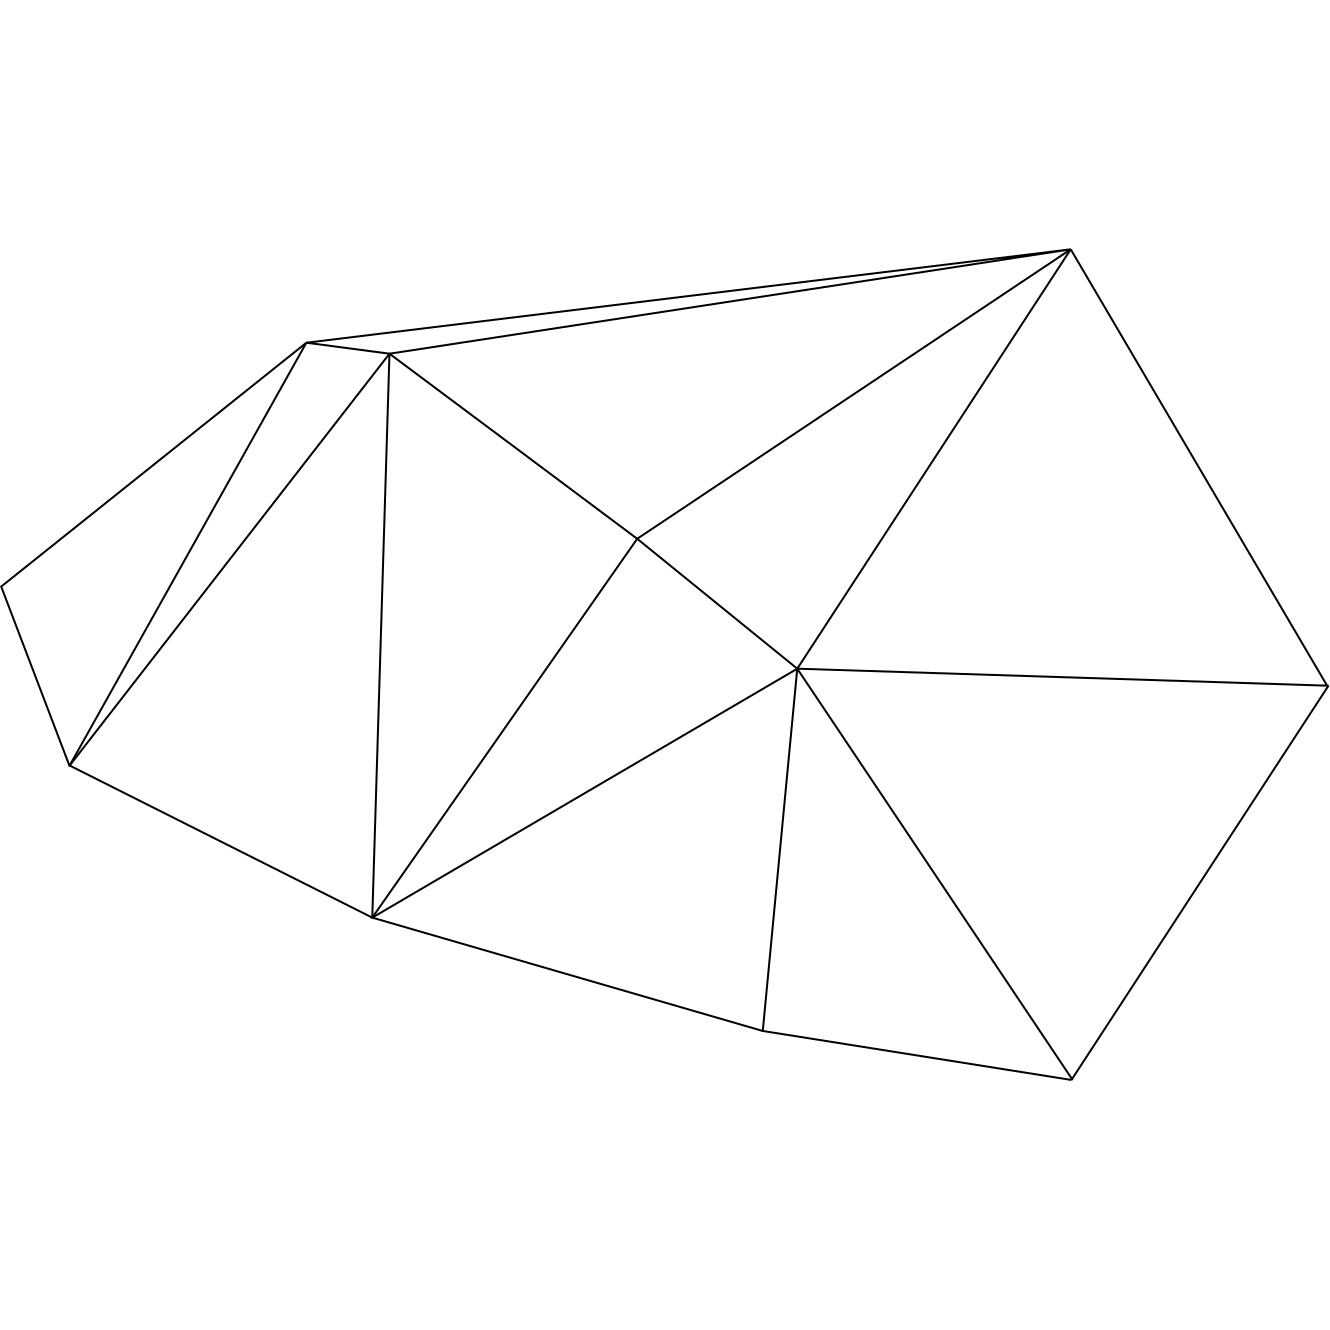
\includegraphics[width=\linewidth]
		{data/synthetic_meshes/random_circle_tessellation_Dirac_delta_1_v11_f12_wireframe.png}
		\caption{$r=1$, $p=11$, wireframe}\label{fig:rcirc.a}
	\end{subfigure}
	\begin{subfigure}[b]{0.32\linewidth}
		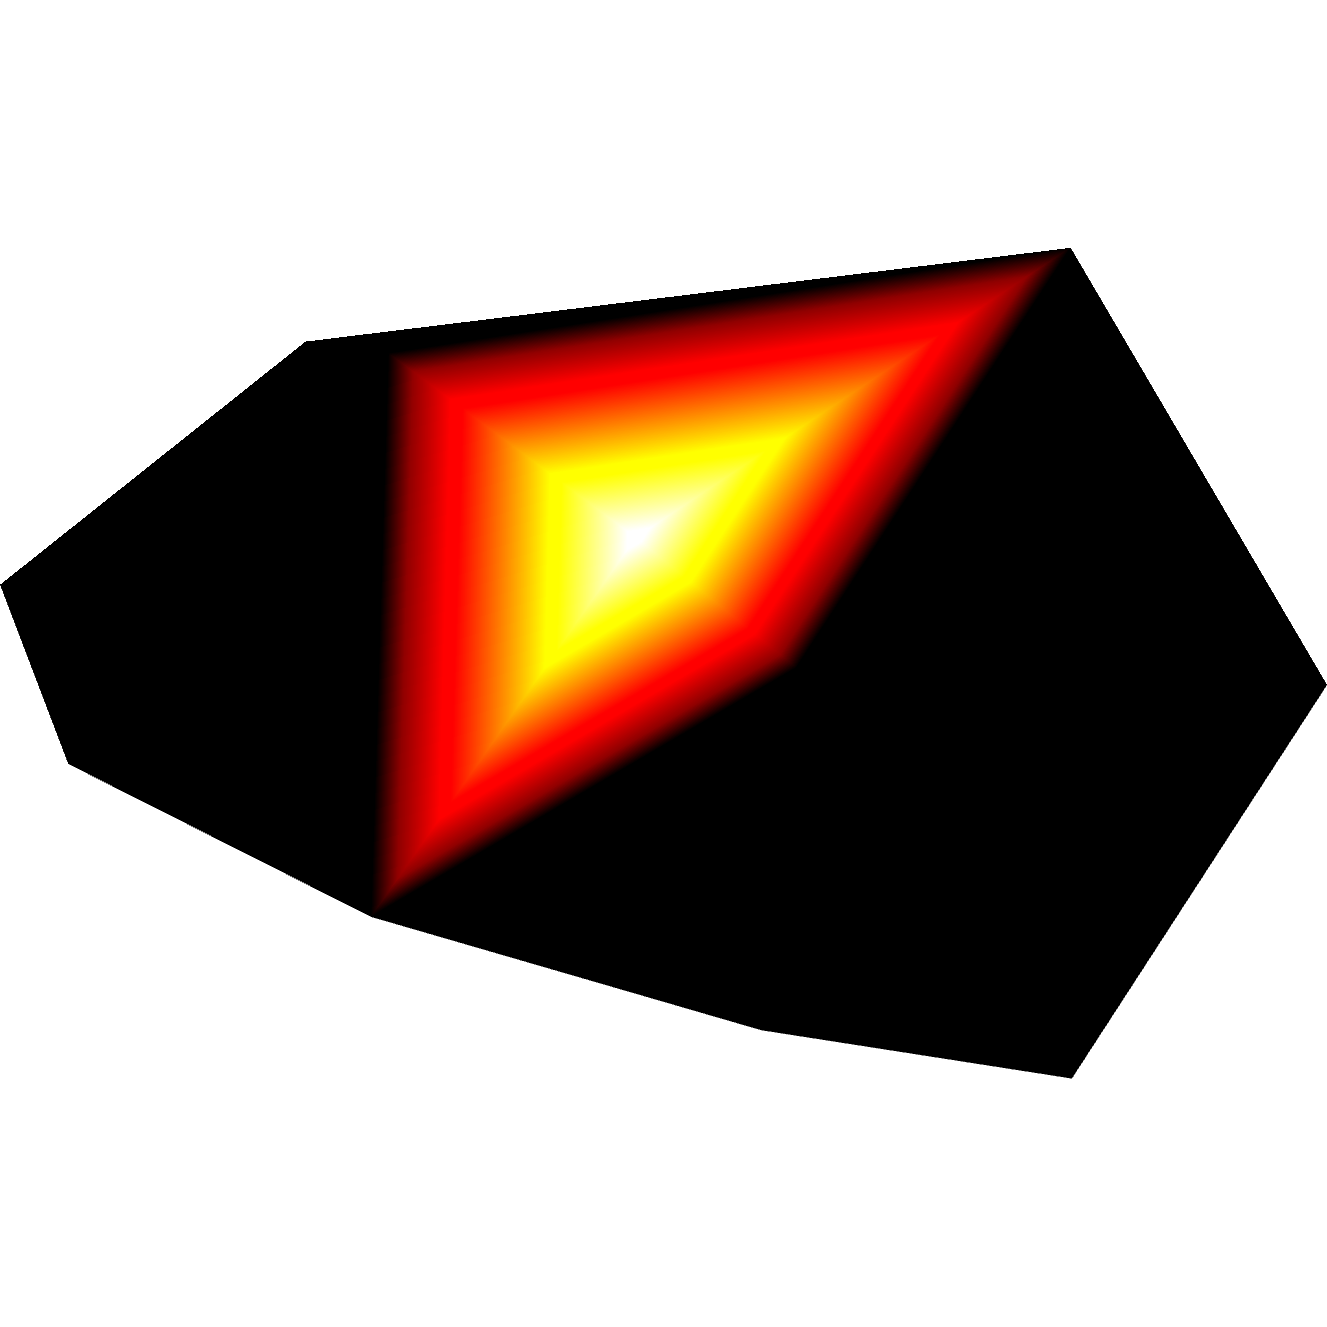
\includegraphics[width=\linewidth]
		{data/synthetic_meshes/random_circle_tessellation_Dirac_delta_1_v11_f12_funcvals_0iter.png}
		\caption{$r=1$, $p=11$, $c=0$}\label{fig:rcirc.c}
	\end{subfigure}
	\begin{subfigure}[b]{0.32\linewidth}
		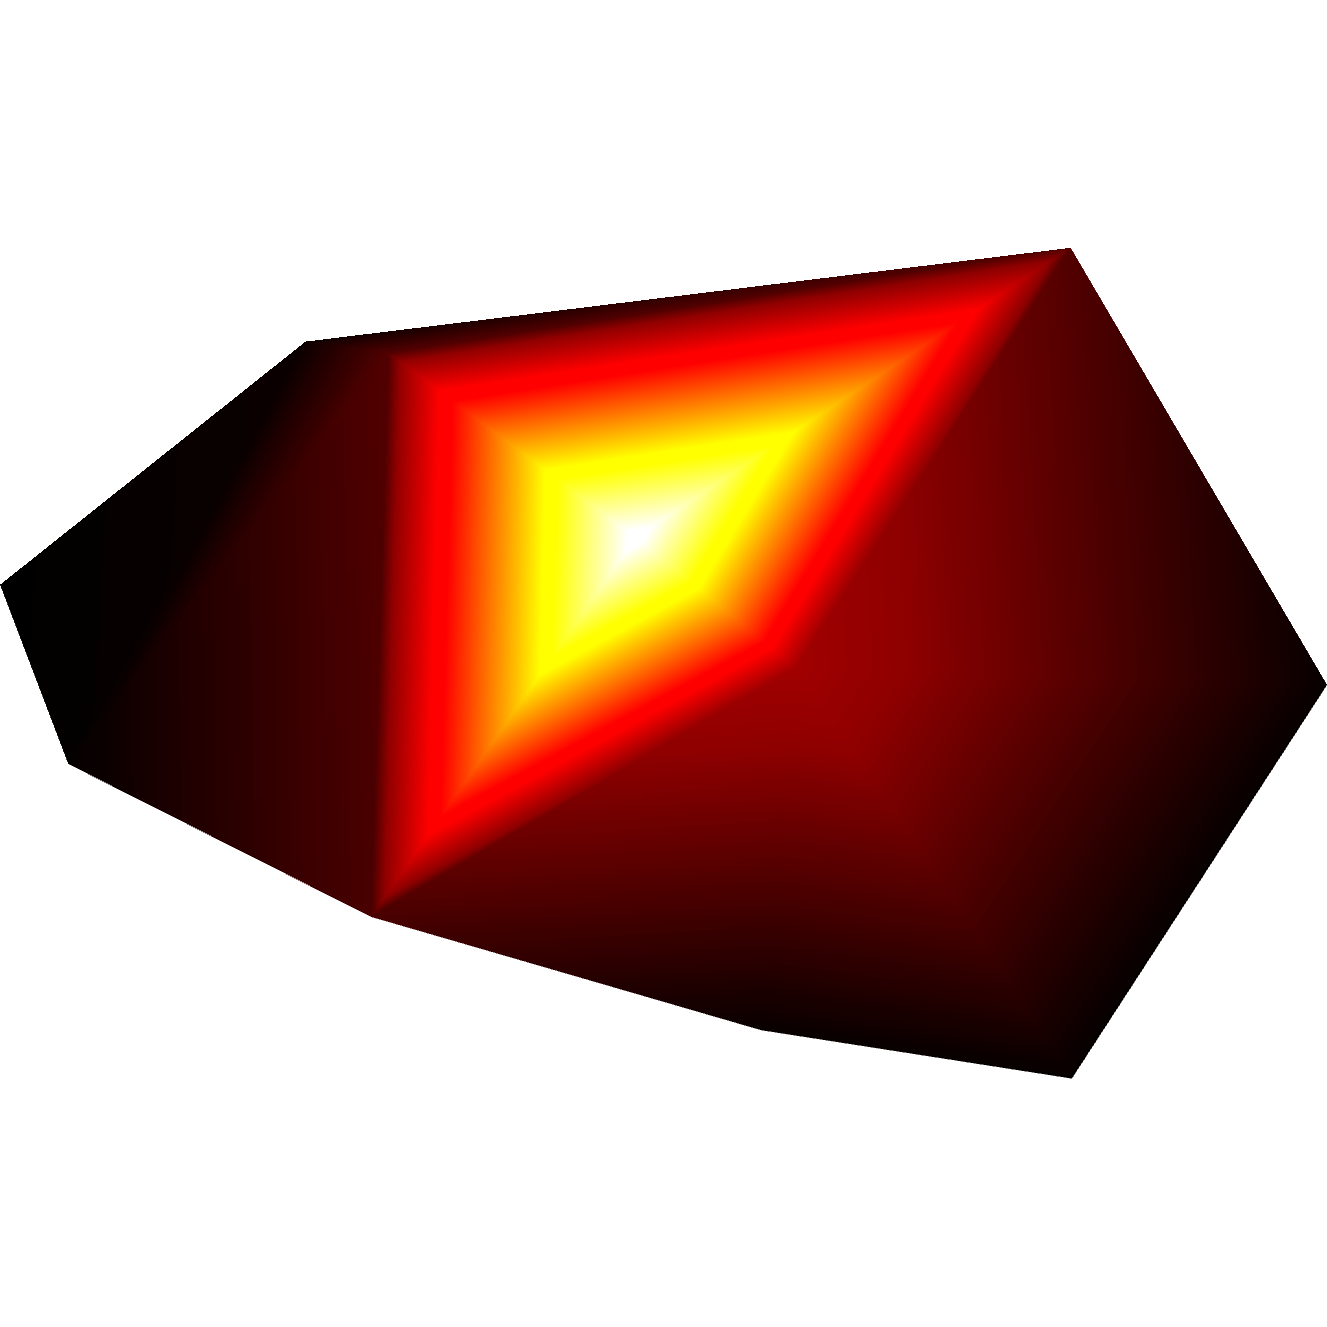
\includegraphics[width=\linewidth,]
		{data/synthetic_meshes/random_circle_tessellation_Dirac_delta_1_v11_f12_funcvals_2iter.png}
		\caption{$r=1$, $p=11$, $c=2$}\label{fig:rcirc.e}
	\end{subfigure}

	\bigskip
	\begin{subfigure}[b]{0.32\linewidth}
		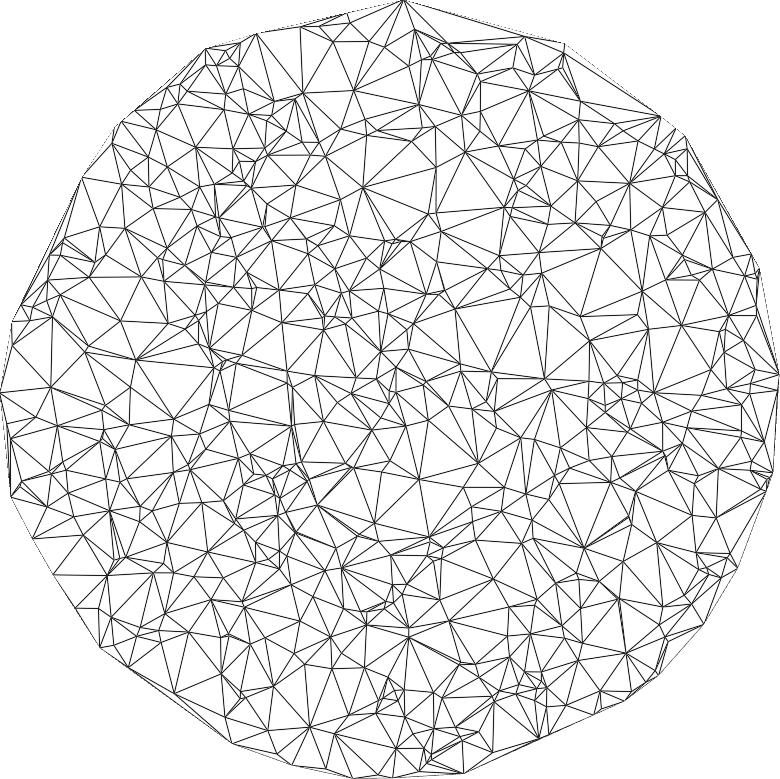
\includegraphics[width=\linewidth]
		{data/synthetic_meshes/random_circle_tessellation_Dirac_delta_10_v641_f1252_wireframe.png}
		\caption{$r=10$, $p=641$, wireframe}\label{fig:rcirc.b}
	\end{subfigure}
	\begin{subfigure}[b]{0.32\linewidth}
		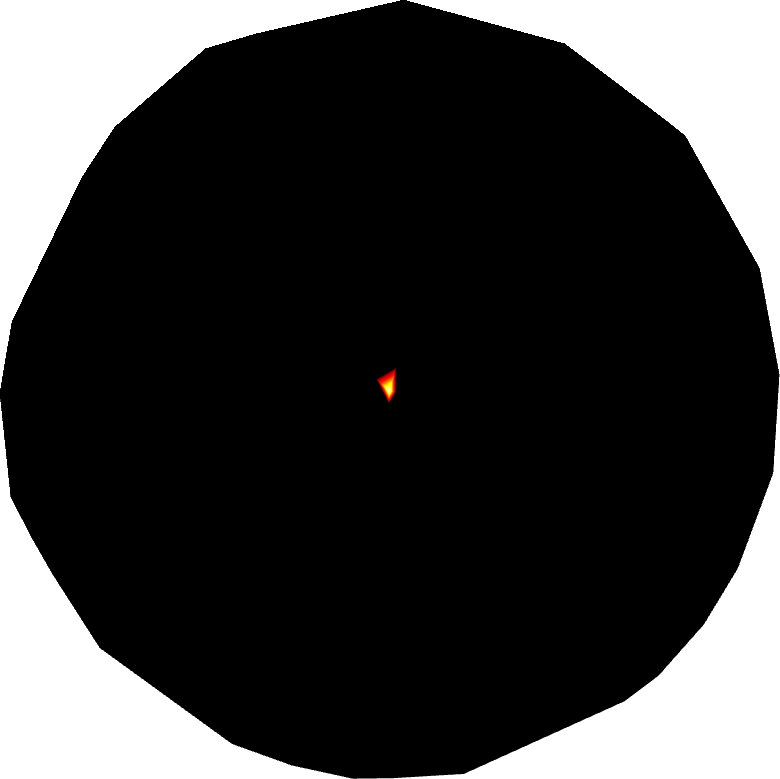
\includegraphics[width=\linewidth]
		{data/synthetic_meshes/random_circle_tessellation_Dirac_delta_10_v641_f1252_funcvals_0iter.png}
		\caption{$r=10$, $p=641$, $c=0$}\label{fig:rcirc.d}
	\end{subfigure}
	\begin{subfigure}[b]{0.32\linewidth}
		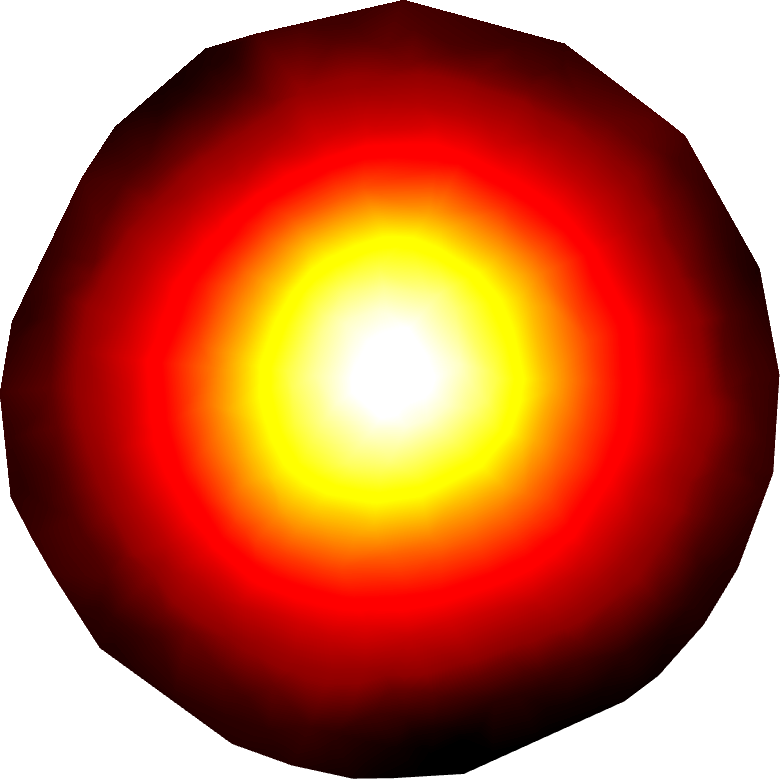
\includegraphics[width=\linewidth]
		{data/synthetic_meshes/random_circle_tessellation_Dirac_delta_10_v641_f1252_funcvals_10000iter.png}
		\caption{$r=10$, $p=641$, $c=10^4$}\label{fig:rcirc.f}
	\end{subfigure}
\end{figure}

